\documentclass{article}
\usepackage[utf8]{inputenc}
 \usepackage{amsmath}
 \usepackage{amssymb}
 \usepackage{graphicx}



\begin{document}
\section*{Arrow matrix x vector multiplication}
We are given the following code segment
\begin{figure}[!hbt]
    \centering
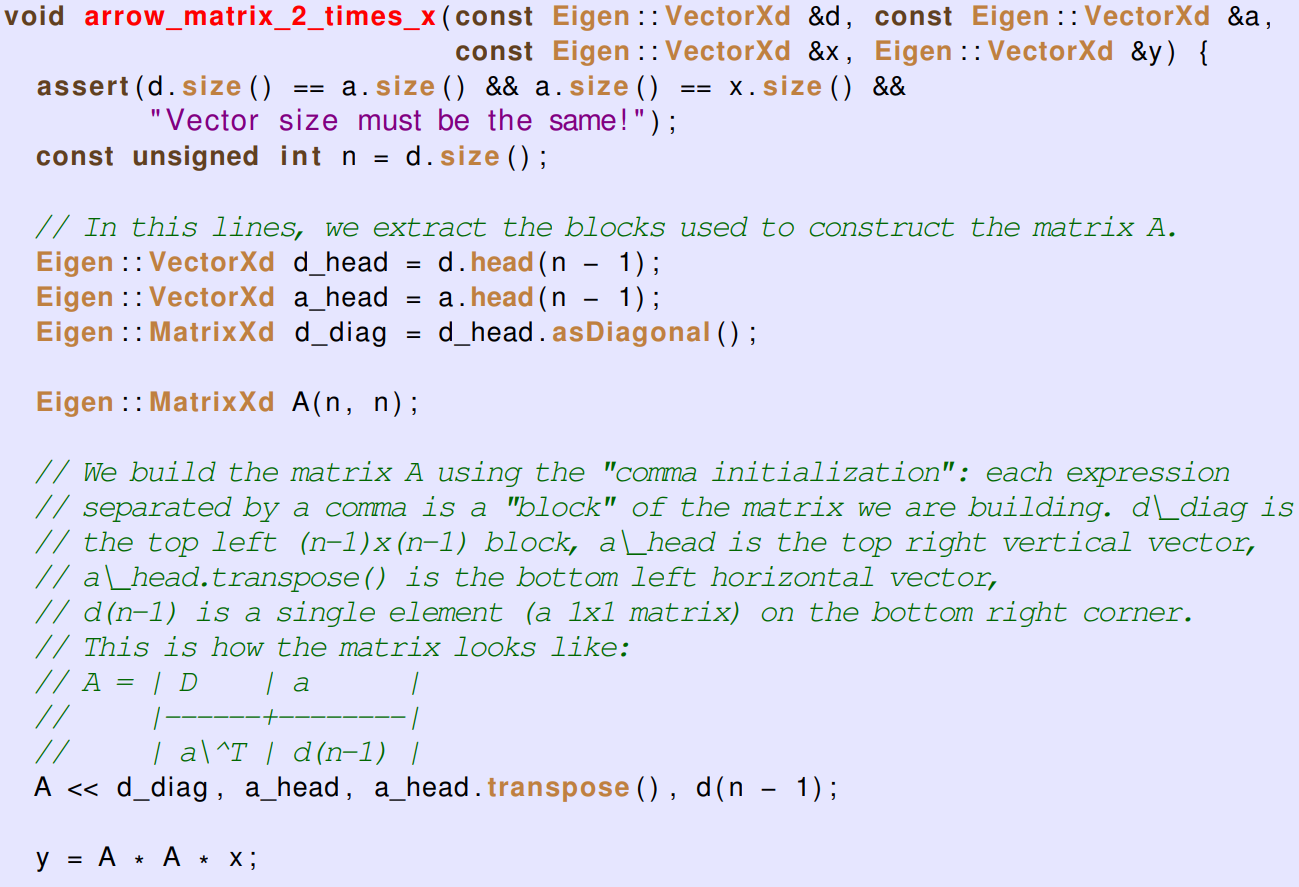
\includegraphics[width=1.0\linewidth]{Code1_1.png}
\end{figure}
An arrow matrix $\mathbf{A}\in \mathbb{R}^{n,n}$ is constructed given two vectors $\mathbf{a}\in \mathbb{R}^{n}$ and $\mathbf{d}\in \mathbb{R}^{n}$. The matrix is then squared and multiplied with a vector $\mathbf{x}\in \mathbb{R}^{n}$.
\subsection*{1-1.a} We are now tasked to sketch the pattern of the nonzero entries of the matrix $\mathbf{A}$ created in the above function, for general vectors $\mathbf{d} = \left[d_{1}, \dots, d_{n}\right]^{\mathsf{T}}$ and $\mathbf{a} = \left[a_{1}, \dots a_{n}\right]^{\mathsf{T}}$. We have the following
\begin{equation*}
    \text{d\_diag} = 
    \begin{bmatrix}
       d_{1} & & \\
       & \ddots & \\
       & & d_{n-1}
    \end{bmatrix}
    \qquad
    \text{a\_head} = 
    \begin{bmatrix}
    a_{1} \\
    \vdots \\
    a_{n-1}
    \end{bmatrix}
\end{equation*}
Hence putting this together (\verb|<<| is overloaded to support block insertions, we get
\begin{equation*}
    \mathbf{A} = 
    \begin{bmatrix}
    d_{\text{diag}} & a_{\text{head}} \\
    a_{\text{head}}^{\mathsf{T}} & d_{n}
    \end{bmatrix} = 
    \begin{bmatrix}
        d_{1} & & & a_{1} \\
           &\ddots& &\vdots \\
         &  & d_{n-1}& a_{n-1}\\
        a_{1} & \dots & a_{n-1}& d_{n}
    \end{bmatrix}
\end{equation*}
We can see that this is an arrow matrix.

\pagebreak 

\subsection*{1-1.b}
We are given the following log-log plot for the timings of the function \verb|arrow_matrix_2_times_x|.
\begin{figure}[!hbt]
    \centering
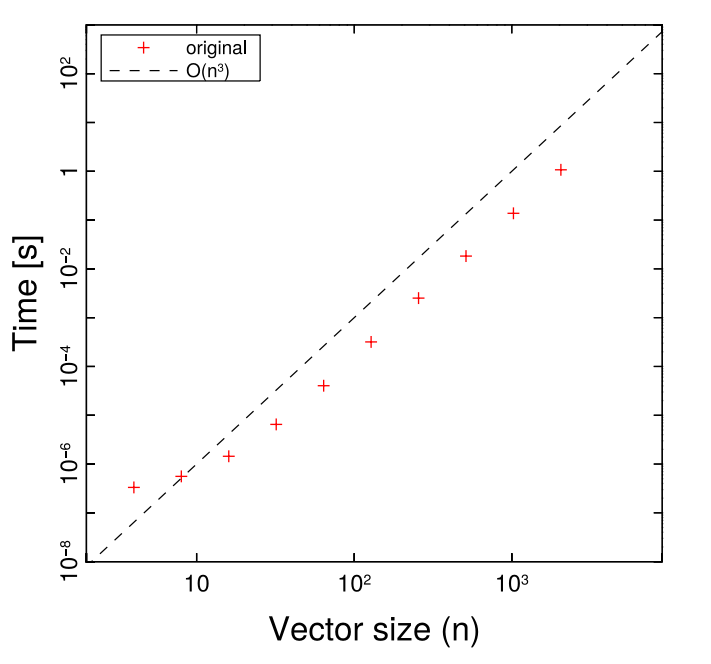
\includegraphics[width=0.5\linewidth]{Timings1_1.png}
\end{figure}

We know need to remember the section on arrow matrices and how multiplying can produce different patterns and that the product of two sparse matrices does not have to be sparse.

\begin{figure}[!hbt]
    \centering
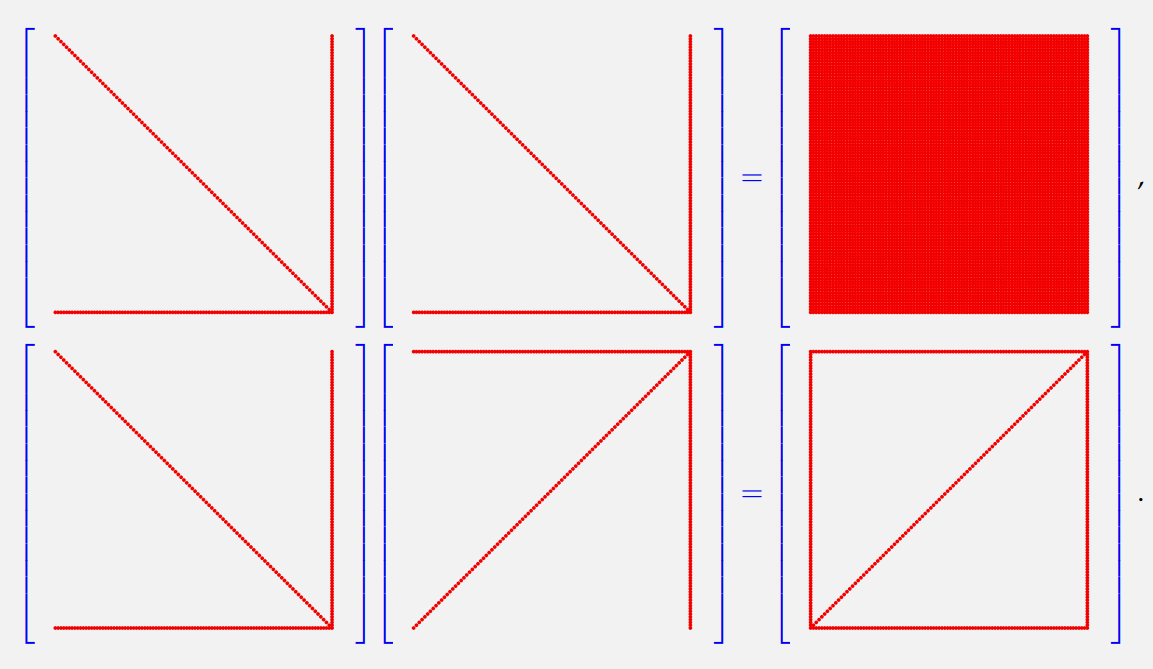
\includegraphics[width=0.7\linewidth]{ArrowMultiplication.png}
\end{figure}

\noindent In our case the above pattern applies, as we multiply $\mathbf{A}$ with itself (\verb|A * A * x| is evaluated as \verb|(A * A) * x| as per usual). We thus get a nonzero result for all $n^{2}$ entries of the matrix of which each takes $\mathcal{O}\left(n\right)$ time to compute. Hence we get an asymptotic runtime of $\mathcal{O}\left(n^{3}\right)$ in the log-log plot.

\pagebreak

\subsection*{1-1.c} 
We are now tasked with writing an efficient implementation of the above code. Let us first rewrite the expression using
\begin{equation*}
    \mathbf{A}^{2}\mathbf{x} = \mathbf{A} \left(\mathbf{A}\mathbf{x}\right)
\end{equation*}
Let us look at the structure the matrix-vector product ($\mathbf{A}\mathbf{x}$) produces, we will call $x_{\text{head}} = \left[x_{1}, \dots, x_{n-1}\right]$
\begin{align*}
    \begin{bmatrix}
        d_{1} & & & a_{1} \\
           &\ddots& &\vdots \\
         &  & d_{n-1}& a_{n-1}\\
        a_{1} & \dots & a_{n-1}& d_{n}
    \end{bmatrix}
    \begin{bmatrix}
        x_{1} \\
        \vdots \\
        x_{n-1} \\
        x_{n}
    \end{bmatrix} &= 
    \begin{bmatrix}
        d_{1}x_{1} + a_{1}x_{n} \\
        d_{2}x_{2} + a_{2}x_{n} \\
        \vdots \\
        d_{n-1}x_{n-1} + a_{n-1}x_{n} \\
        a_{1}x_{1} + \dots a_{n-1}x_{n-1} + d_{n}x_{n}
    \end{bmatrix} \\
    &= \underbrace{x_{n}\cdot\begin{bmatrix}
        a_{1} \\
        a_{2} \\
        \vdots \\
        a_{n-1} \\
        a_{n}
    \end{bmatrix}}_{\mathrm{ax}\: * \:x\left(n-1\right)} + \underbrace{\begin{bmatrix}
        d_{1}x_{1} \\
        d_{2}x_{2} \\
        \vdots \\
        d_{n-1}x_{n-1} \\
        d_{n}x_{n}
    \end{bmatrix}}_{\mathrm{cwiseProduct}} + \begin{bmatrix}
        0 \\
        0 \\
        \vdots \\
        0 \\
        \underbrace{a_{1}x_{1} + \dots a_{n-1}x_{n-1}}_{\mathrm{dot}}
    \end{bmatrix}
\end{align*}

\noindent Let us go through the code line per line. A functor as we implemented in the first line has the following form
\begin{equation*}
    \text{auto name} = \underbrace{\left[c_{1}, \dots, c_{n}\right]}_{\text{captures}}\underbrace{\left(p_{1}, \dots, d_{m}\right)}_{\text{parameters}} \rightarrow \text{return type} \left\{ \text{ functor body } \right\};
\end{equation*}
The above is a lambda expression which we often refer to as a functor. Captures are given to a functor to ensure that the functor can access the objects being capture even from outside where they are defined. We can an object \verb|example| capture by value using \verb|[example]| or by reference using \verb|[&example]|, reference capturing makes more sense for most object and we use value capturing mostly for primitive types which are not expensive to pass by creating a copy. The parameters is what we call the functor with, here we would call \verb|name(p1, ..., pn)| and the functor would execute the functor body and return the type specified after $\rightarrow$.
\noindent The first line of the functor makes use of the Eigen type \verb|Eigen::ArrayXd|, this allows for using operations like \verb|*|, \verb|+|, \verb|/|, \verb|.pow()|, \verb|.exp()| and many more directly on each element of the array directly. The method \verb|head(size)| gives read / write access to the top size elements of the vector. We use \verb|cwiseProduct| to take a coefficient wise product meaning we do
 \begin{equation*}
     \mathrm{x.cwiseProduct(y)} \Longleftrightarrow \begin{bmatrix}
         x_{1}y_{1} \\
         x_{2}y_{2} \\
         \vdots \\
         x_{n}y_{n}
     \end{bmatrix}
 \end{equation*}

\noindent We then make use of \verb|dot| which does compute the inner product of two vectors, i.e.
\begin{equation*}
    \mathrm{x.dot(y)} \Longleftrightarrow x^{\mathsf{T}}y
\end{equation*}

The following figure shows the code we mentioned.

\begin{figure}[!hbt]
    \centering
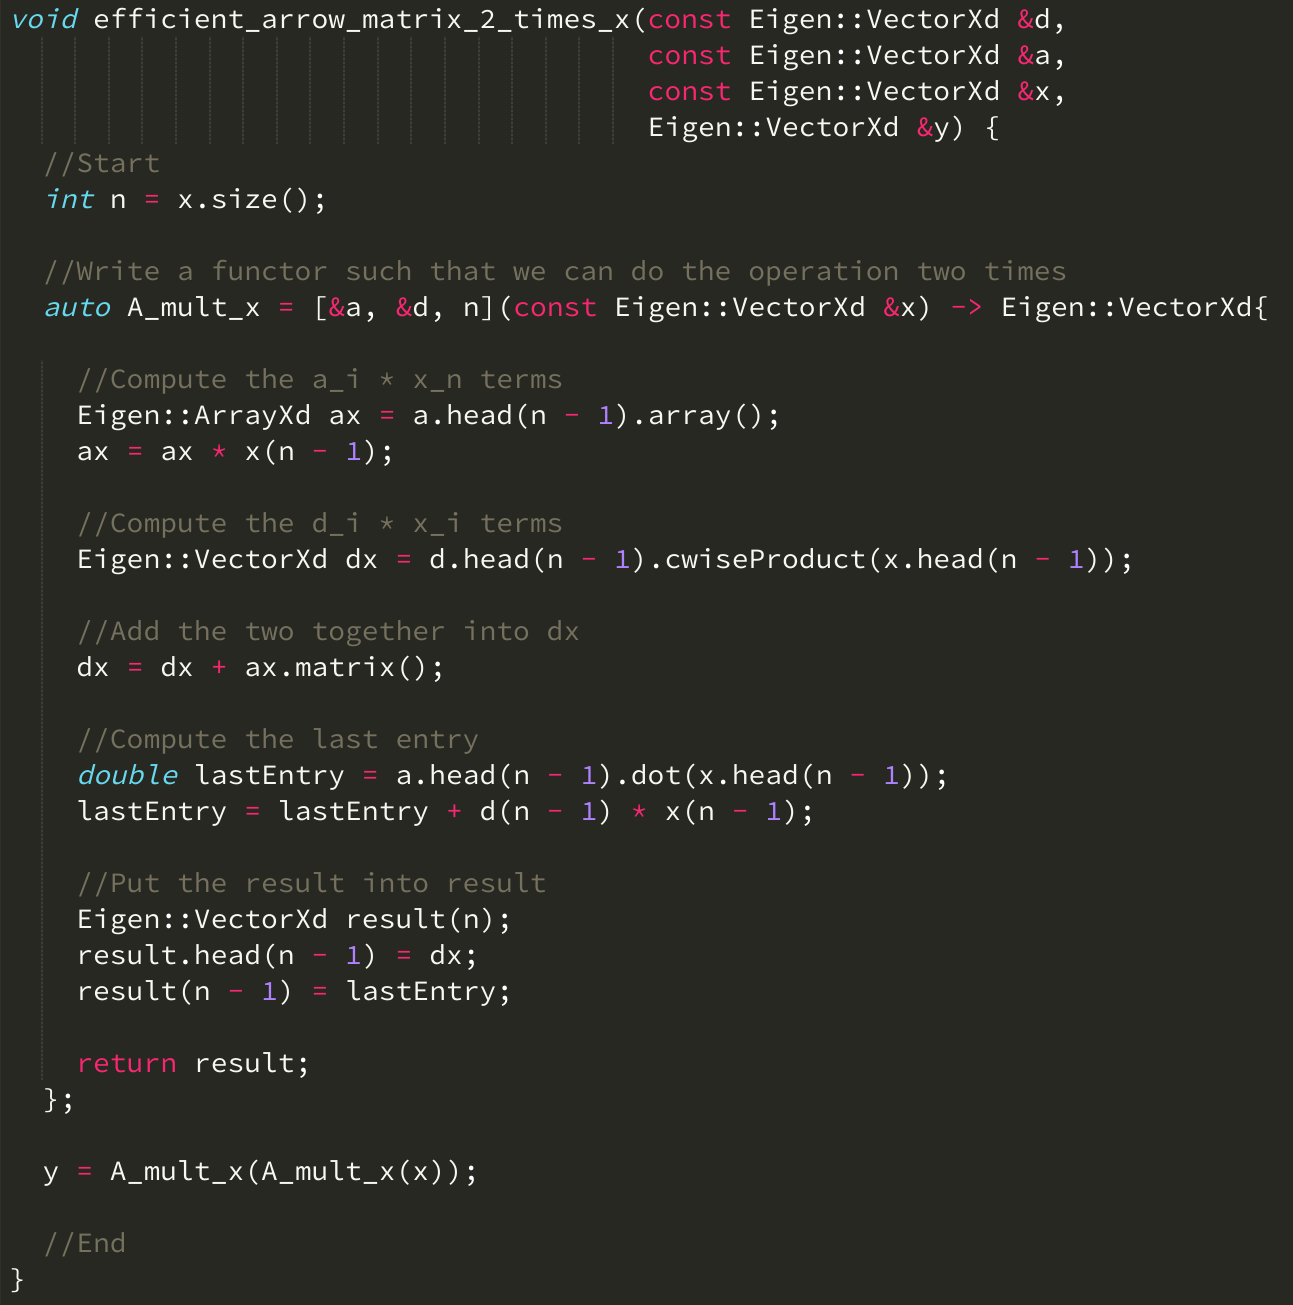
\includegraphics[width=1.0\linewidth]{Code1_1c.png}
\end{figure}

\pagebreak


\subsection*{1-1.d}
We are tasked with stating the asymptotic complexity of our code. Let us go through the code. Initializing an array of size $n-1$ takes $\mathcal{O}\left(n\right)$ The operation \verb|*| we do in the line below that does coefficient-wise multiplication with a factor, hence this also takes $\mathcal{O}\left(n\right)$, we then do a \verb|cwiseProduct|, which does $n$ coefficient operations overall taking $\mathcal{O}\left(n\right)$, the addition done for \verb|dx| is also done in $\mathcal{O}\left(n\right)$ as we just add two arrays coefficient wise. The dot product does $\mathcal{O}\left(n\right)$ multiplications and $\mathcal{O}\left(n\right)$ additions and storing the result takes $\mathcal{O}\left(n\right)$ as well. Hence the functor computes the result in $\mathcal{O}\left(n\right)$. Doing this two times overall gives us the final time complexity of $\mathcal{O}\left(n\right)$.

\subsection*{1-1.e}
This part of the exercise goes in depth on how the \verb|Timer| works and one should use the structured given in future exercises where we need a timer.
\end{document}
